%
% Header die benutzt werden sollen
%
\documentclass[
  pdftex,
  fontsize=12pt,          % Schriftgroesse
  DIV10,                  % Angabe bzgl Bestimmung der Seitenabstaende
  ngerman,                % fuer Umlaute, Silbentrennung etc.
  paper=a4,               % Papierformat
  twoside=false,          % einseitiges Dokument
  titlepage,              % es wird eine Titelseite verwendet
  parskip=half,           % Abstand zwischen Absaetzen (halbe Zeile)
  headings=normal,        % Groesse der Ueberschriften verkleinern
  listof=nochaptergap,    % Verzeichnisse im Inhaltsverzeichnis auffuehren.
  bibliography=totoc,     % Literaturverzeichnis im Inhaltsverzeichnis auffuehren
  index=totoc,            % Index im Inhaltsverzeichnis auffuehren
  captions=tableheading,  % Beschriftung von Tabellen oberhalb ausgeben
  bookmarksopen,
  bookmarksnumbered,
  final                   % Status des Dokuments (final/draft)
]{scrreprt} 

\usepackage[T1]{fontenc}
\usepackage[utf8]{inputenc}
\usepackage[ngerman]{babel}
\usepackage{palatino}

% Zeilenabstand
\usepackage[onehalfspacing]{setspace}

% Code
\usepackage{listings}
\lstdefinestyle{sharpc}{float,
	language=[sharp]C, 
	frame=single,  
	keywordstyle=\bfseries\color{green!40!black},
	commentstyle=\itshape\color{purple!40!black},
	identifierstyle=\color{blue},
	stringstyle=\color{orange}, 
	showstringspaces=false, 
	showspaces=false, 
	numbers=left, 
	captionpos=b, 
	belowcaptionskip=4pt,
	basicstyle=\ttfamily}

%Tabellen
\usepackage{array}
\usepackage{tabularx}
\usepackage{supertabular}
\usepackage{longtable}

%Grafiken
\usepackage[pdftex]{graphicx}
\usepackage{wrapfig}
\usepackage[svgnames]{xcolor}
\usepackage{float}
\usepackage{pdfpages}

%Sprache und Anführungszeichen
\usepackage[babel,german=quotes]{csquotes}
\usepackage{eurosym}

%Abstände
\usepackage[left=2.5cm, right=2.5cm, top=2.5cm, bottom=2.5cm ]{geometry}

% Pakete um Textteile drehen zu können, oder eine Seite Querformat anzeigen kann.
\usepackage{rotating}
\usepackage{lscape}

%Literaturverweise
\usepackage[style=numeric, backend=biber, citestyle=numeric, dashed=false]{biblatex}

% Hurenkinder und Schusterjungen verhindern
% http://projekte.dante.de/DanteFAQ/Silbentrennung
\clubpenalty=10000
\widowpenalty=10000
\displaywidowpenalty=10000

%Abkürzungsverzeichnis
\usepackage[printonlyused]{acronym}

% Fussnoten
\usepackage[hang, multiple, stable]{footmisc}

\usepackage[%
%	pdftitle={\pdftitel},
%	pdfauthor={\autor},
%	pdfsubject={\arbeit},
%	pdfcreator={pdflatex, LaTeX with KOMA-Script},
%	pdfpagemode=UseOutlines, % Beim Oeffnen Inhaltsverzeichnis anzeigen
%	pdfdisplaydoctitle=true, % Dokumenttitel statt Dateiname anzeigen.
%	pdflang=de % Sprache des Dokuments.
]{hyperref}
\usepackage[all]{hypcap}


% Nummerierung ohne Kapitel-Nr.
\usepackage{chngcntr}
\counterwithout{figure}{chapter}
\counterwithout{equation}{chapter}
\counterwithout{footnote}{chapter}
\counterwithout{table}{chapter}
%
% EOF
%
\addbibresource{lib.bib}
\begin{document}
\renewcommand{\bibname}{Literaturverzeichnis}  

%Glossar

\setlength{\parindent}{0mm}

%mindestens 3 Zeilen auf der Seite
\widowpenalties 3 10000 10000 100
\clubpenalties 3 10000 10000 100 

%Stil der Quellangaben
%\bibliographystyle{alphadin}

%Deckblatt
%
% Deckblatt
%

\begin{titlepage}

	\begin{center}
		% Logos der Firma und DHBW
		\vspace*{0cm}
		%\includegraphics[width=8cm]{images/firma}
		\hfill
		%\includegraphics[width=6cm]{images/dhbw-logo}\\ [3cm]
		%Titel, Typ der Arbeit, Studiengang
		{\Large \textbf{Titel} } 	\\ [2cm]
		{\Large  \scshape \textbf{Studienarbeit}}	\\ [2cm]
		{\large des Studiengangs Angewandte Informatik}	\\ [0.5cm]
		{\large an der Dualen Hochschule Baden-Württemberg Karlsruhe}	\\[0.5cm]
		
		
		{\large von} 	\\ [0.5cm]
		%Autor und Abgabedatum
		{\large \bfseries \textbf{Mehmet Ali Incekara \& Tom Wolske}}	\\ [1cm]
		{\large Abgabedatum \today}
		\vfill
	\end{center}
	
	\begin{tabular}{l@{\hspace{2cm}}l}
	\textbf{Bearbeitungszeitraum}			&	12 Wochen		\\
	\textbf{Matrikelnummer}					&	12345678 \& 1156973		\\
	\textbf{Kurs}							&	TINF14B2			\\
	\textbf{Gutachter der Studienakademie}	&	Prof. Dr. Kay Berkling	\\
	\end{tabular}

\end{titlepage}

%
% EOF
%

\renewcommand{\thepage}{\Roman{page}}
\setcounter{page}{1}
% Formale Erklärungen
%\thispagestyle{empty}

\section*{Erklärung}
% Seite 8
% http://studium.ba-bw.de/fileadmin/media/allgemein/bestimmungen/btechnik/richtlinien/Richtlinien_Praxismodule_Studien_und_Bachelorarbeiten_2011.pdf
\vspace*{2em}

Gemäß \S 5 (2) der \enquote{Studien- und Prüfungsordnung DHBW Technik} vom 18. Mai 2009 erkläre ich hiermit,
\begin{enumerate}
\item dass ich die vorliegende Arbeit selbstständig verfasst und keine anderen als die
angegebenen Quellen und Hilfsmittel verwendet habe. 
\item dass die Übernahme von Zitaten und Gedankengut anderer Autoren gekennzeichnet wurde.
\item dass die eingereichte elektronische Fassung exakt mit der schriftlichen übereinstimmt.
\item dass ich die Projektarbeit keiner externen Prüfung vorgelegt habe.
\end{enumerate}

\vspace{3em}

\begin{tabular}{lp{2em}l}
 Karlsruhe, den \today  && \hspace{7cm} \\\cline{1-1}\cline{3-3}
 Ort, Datum     &&  Tom Wolske
\end{tabular} 

\begin{tabular}{lp{2em}l}
 Karlsruhe, den \today  && \hspace{7cm} \\\cline{1-1}\cline{3-3}
 Ort, Datum     &&  Mehmet Ali Incekara
\end{tabular} 

%Abstract

% Inhaltsverzeichnis

\tableofcontents
\newpage
\newpage
\phantomsection
\addcontentsline{toc}{chapter}{Abkürzungsverzeichnis}
\chapter*{Abkürzungsverzeichnis}
\begin{acronym}[SDK]

\acro{SDK}{Software Development Kit}

\end{acronym}
\newpage
\listoffigures
%\addcontentsline{toc}{chapter}{Abbildungsverzeichnis}
%\newpage
%\listoftables
%\addcontentsline{toc}{chapter}{Tabellenverzeichnis}
\newpage
\counterwithout{lstlisting}{chapter}
\lstlistoflistings
%\addcontentsline{toc}{chapter}{Listings}

%--> Speichern der Zahl fürs umsetzten zurück auf römische 
\newcounter{SeitenzahlSpeicher}
\setcounter{SeitenzahlSpeicher}{\value{page}}

%\newpage
\newpage

%Arabische Nummerierung
\renewcommand{\thepage}{\arabic{page}}
\setcounter{page}{1}
	
%Kapitel
\chapter{Einleitung}

Spiele, jeder kennt sie und spielt regelmäßig welche. Sie sind ein fester Bestandteil unserer Kultur und das schon seit tausenden Jahren. Die ersten Gesellschaftsspiele wurden noch im Sand mit Stöcken oder Steinen gespielt. Eines der frühesten Spiele wird auch heutzutage noch gespielt, dabei handelt es sich um Mühle, ein Spiel welches die Ägypter vor bereits 3000 Jahren gespielt haben.\footnote{vgl. gesellschaftsspiele.de \cite{spiele} (2015)} Spiele haben sich seit dem jedoch weiterentwickelt und dienen heutzutage nicht nur zum munteren Zeitvertreib. 

Ob als Brett, Karten oder Glücksspiel, Spiele sind überall zu finden und jeder kann sie spielen. Seit 1972 entwickeln sich darüber hinaus weitere Spiele, Videospiele. Sie nutzen die immer größer werdende Rechenleistung von Computern aus, um uns immer realistisch aussehender Spiele zu liefern. 
Um den Überblick über die Vielzahl an Videospielen zu behalten, haben sich in den letzten Jahren verschiedene Plattformen etabliert, die versuchen dem Nutzer das zu bieten, was sie suchen. Dabei stellen diese viele verschiedene Arten von Spielen für die Gamer bereit, die einen beim Spielen die Zeit vergessen lassen. Beispiele für solche Plattformen sind unter anderem Steam, Uplay oder Origin.

Allerdings können Spiele uns nicht nur die Zeit vergessen lassen und für heitere Stunden sorgen, sie können uns auch Wissen vermitteln. Sei es beispielsweise durch eine Geschichte die sich real abgespielt hat, wie der erste Weltkrieg. Dieses Wissen wird unterbewusst an den Nutzer vermittelt, ohne das er aktiv versucht dieses zu lernen.

Für diesen Zweig hat sich eine eigene Branche entwickelt, welche sich mit Lernspielen befasst und versucht uns, über Videospiele, neues Wissen zu vermitteln. Viele dieser Spiele nutzen bekannte Figuren, welche die Kinder aus dem Fernsehen kennen, um dieses Wissen zu vermitteln.

Diese Spiele werden hauptsächlich in den Schulen eingesetzt, um den Kindern wissen spielerisch zu vermitteln. Jedoch profitiert nicht jedes Kind von diesem Vorteil. Sei es, weil die Schule keine Computer hat oder weil das Kind nicht eine Schule besuchen kann. Für diesen Zweck wurde die Plattform Hone\footnote{siehe \url{http://hone-kids.herokuapp.com/}} entwickelt, mit der Kinder, die nicht zur Schule gehen können, die Möglichkeit haben, Wissen zu erlangen. 

\section{Motivation}
Bei Hone handelt es sich um eine Spielplattform auf der sich Kinder, bevorzugt aus Regionen in denen Bildung mangelhaft ist, anmelden können. Auf dieser Web-Plattform gibt es für Kinder die Möglichkeit neue Lernspiele für verschiedene Plattformen herunterzuladen. Zusätzlich gibt es eine Ansicht der gelernten Kompetenzen. 

Dieses Konzept hat zwei wesentliche Nachteile für die Benutzer. Für die Verwendung der Web-Plattform wird ein Computer benötigt und gerade weil Spiele für verschiedene Plattformen angeboten werden können, benötigt das Kind mehrere Geräte. Neben diesen Nachteilen, ist das Aussehen und die Bedienung dieser Plattform nicht reizvoll für Kinder gestaltet.

Mehr Kinder als je zuvor in der Geschichte arbeiten täglich mit immer neueren und besseren technischen mobilen Geräten. Deshalb soll eine mobile Applikation, kurz App, für Smartphones entwickelt werden, in der die Kinder auf spielerischer weise Fortschritte machen. Durch die Umsetzung als App wird den Kindern eine Plattform angeboten, mit welcher sie unabhängig und jederzeit auf die Lerninhalte zugreifen können. Ein weiterer Vorteil ist, dass die Kinder den technischen Umgang mit Smartphones lernen. Die App wird unabhängig von Hone funktionieren und es werden keine Inhalte und Funktionen übernommen.

\section{Ziel der Arbeit}

Das Ziel dieses Projektes ist es den Kindern eine Möglichkeit zu geben, mit der sie jederzeit, überall und einfach auf die Lerninhalte zugreifen und spielerisch neues Wissen erwerben können.

Dabei ist es nicht das Ziel die Lerninhalte direkt in der App abzufragen sondern Lernspiele für Smartphones anzubieten, welche es in korrekter Reihenfolge freizuschalten und zu spielen gilt.

Das Ziel dieser Arbeit ist die Vorgehensweise, Bedingungen, Probleme zu dokumentieren. Mit dieser Dokumentation soll gewährleistet werden, dass dieses Projekt von allen Verstanden wird.

\section{Aufbau der Arbeit}

Die einzelnen Kapitel dieser Arbeit repräsentieren die notwendigen Schritte, das Ziel dieses Projektes zu erreichen.

Bevor überhaupt Anforderungen spezifiziert werden können, müssen zunächst die Ideen und Gründe hinter diesem Projekt beschrieben werden. Das nächste Kapitel behandelt deshalb das Konzept der App. Zudem wird das beschriebene Konzept von anderen Spielkonzepten abgegrenzt, um die Unterschiede klarzustellen.

Im darauf folgendem dritten Kapitel wird das zum Projekt dazugehörende Software Requirements Specifikation behandelt. Dies dient zur Spezifikation der App. Neben funktionalen Anforderungen werden hier auch nicht-funktionale Anforderungen festgeschrieben.

Anschließend wird auf die technischen Grundlagen für die Umsetzung eingegangen. Dabei wird die gewählte Entwicklungsumgebung und weitere notwendigen Technologien beschrieben.

Darauf aufbauend wird im fünften Kapitel die Umsetzung behandelt. Dabei wird auf Besonderheiten und Probleme in der Entwicklungsphase eingegangen. Dafür werden die einzelnen Komponenten der App beschrieben.

Abgeschlossen wird diese Arbeit mit einem Fazit und Ausblick, in dem der weitere Werdegang des Projektes geschildert wird.
\include{chapter/1}
\include{chapter/2}
\chapter{Fazit und Ausblick}
	In diesem letzten Abschnitt wird ein letztes Mal zurückblickend auf das Projekt, die Probleme und den geplanten Features geschaut. Abgeschlossen wird diese Arbeit mit einem Ausblick. 
	
	\section{Fazit}
		Noch einmal das Ziel wiederholen 
	
		Projekt allgemein Fazit
		
		Konkrete Probleme: Spiele, Kontrolle über den Fortschritt (wieso deshalb nicht der geplante Fortschrittanzeige entwickelt wurde sondern nur eine Liste, da eine konkrete Überprüfung nicht möglich war)
		
		Fazit aus UI Evaluation - was anders machen
		
		Vielleicht ein bisschen zu komplex für die am anfang abgezielte Altersgruppe - eher für Kinder ab der 5ten Klasse, die schon fliesend lesen können -- ggf. eine Sprachfunktion einbauen, dass die Texte, die angezeigt werden auch vorgelesen werden
		
		

	\section{Ausblick}
		Webfrontend ...
		
		Eigene Spiele zur Überprüfung, ob der Spieler den Standard erfüllt hat...
		
		weitere Klassen und weiter Fächer, dementsprechend auch neue Spielwelten
		
		Ranking/Multiplayer/...

%Römische Nummerierung --> SeitenzahlSpeicher
\stepcounter{SeitenzahlSpeicher}
\renewcommand{\thepage}{\Roman{page}}
\setcounter{page}{\theSeitenzahlSpeicher}

\setlength
\bibitemsep{12pt}

\printbibliography

%Anhang
\newpage
\newpage
\phantomsection
\addcontentsline{toc}{chapter}{\protect{}Anhang}

\chapter*{Anhang}
\section*{Activity Diagramme}
	\begin{figure}[htbp]
		\centering 
		\label{umlOpenMap}
		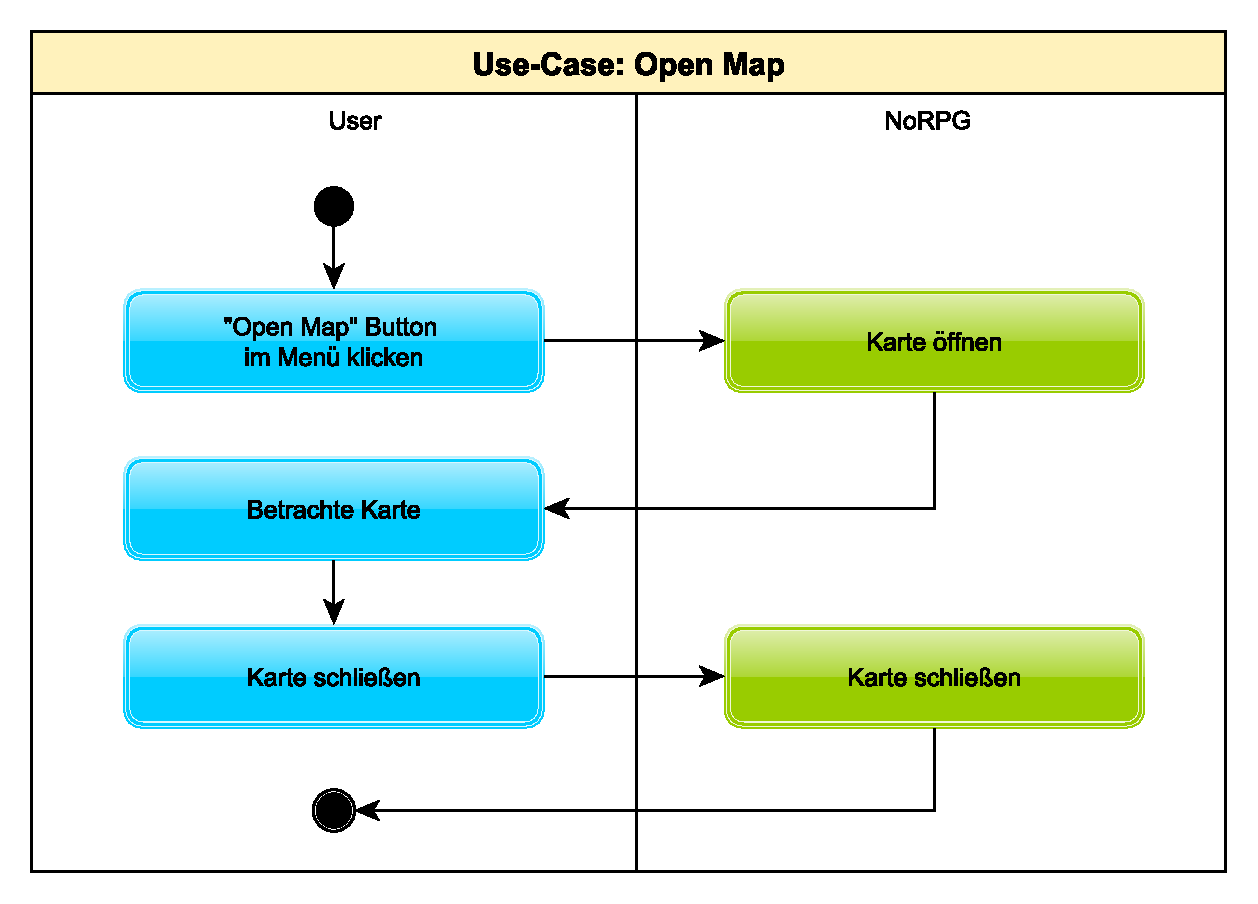
\includegraphics[width=10cm]{pics/OpenMap.pdf}
		\caption{Activity Diagramm: Open Map}
	\end{figure}

	\begin{figure}[htbp]
		\centering 
		\label{umlViewProgess}
		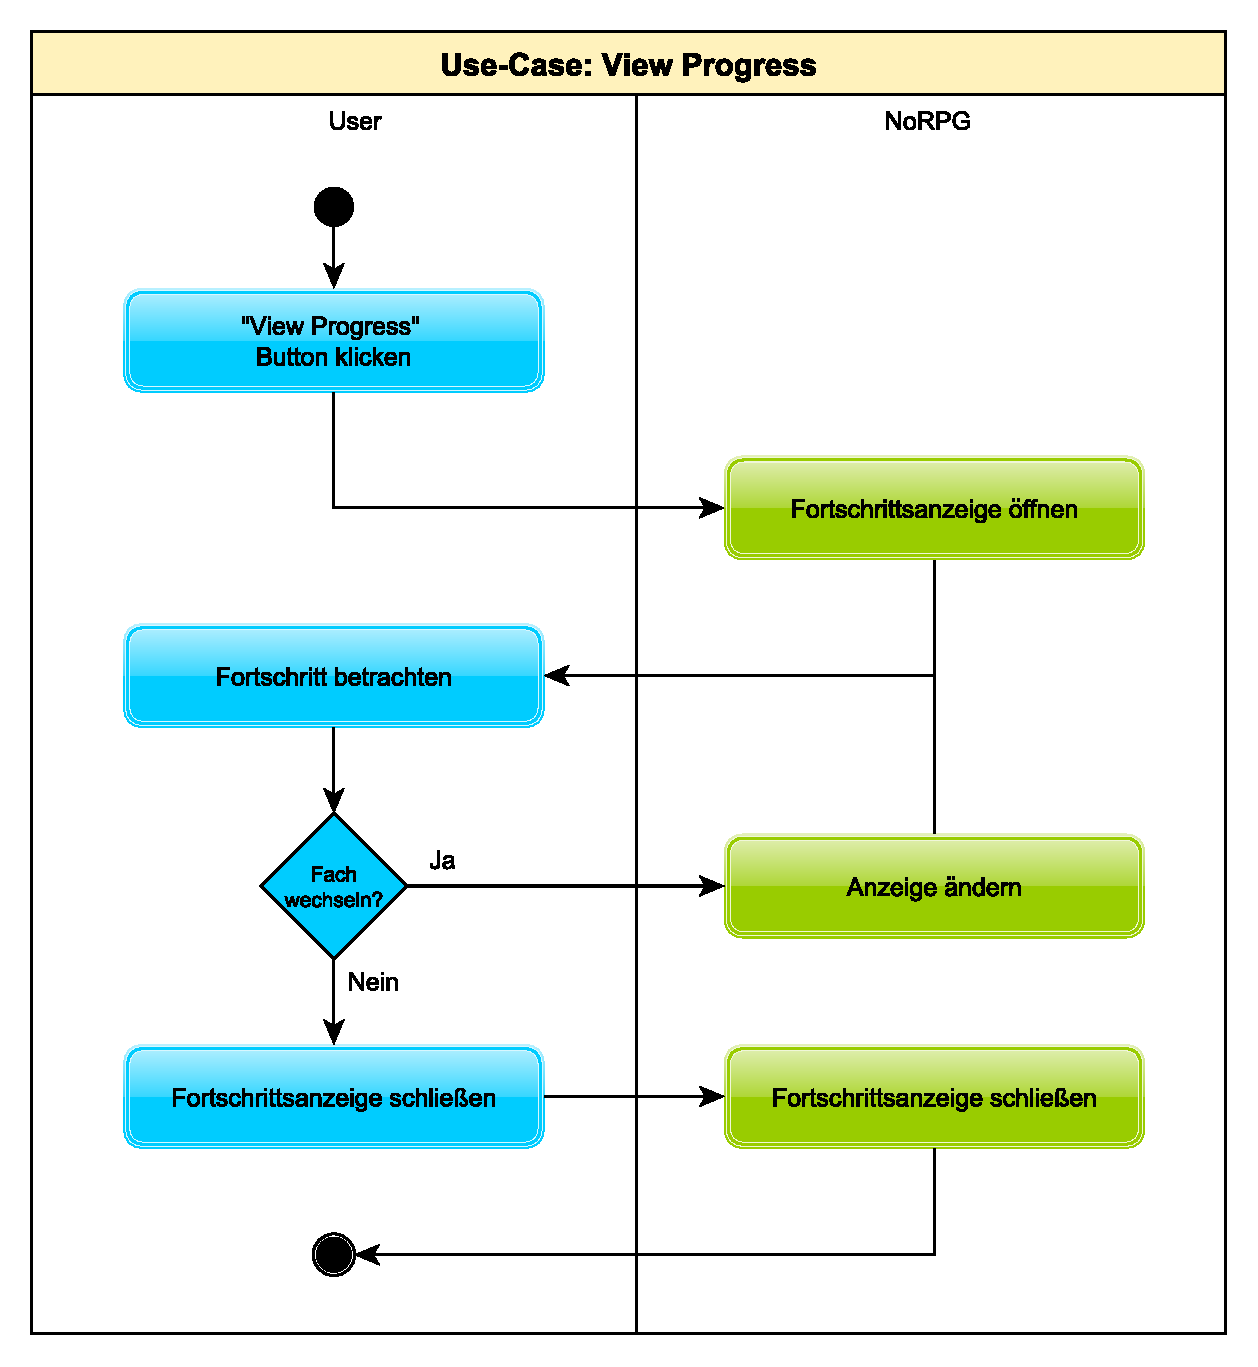
\includegraphics[width=10cm]{pics/ViewProgress.pdf}
		\caption{Activity Diagramm: View Progress}
	\end{figure}

\end{document}